\documentclass{article}

% ICLR 2026 style
\usepackage{iclr2026_conference,times}
\usepackage{url}
\usepackage{booktabs}
\usepackage{amsmath}
\usepackage{amssymb}
\usepackage{graphicx}
\usepackage{multirow}
\usepackage{xcolor}
\usepackage{hyperref}
\usepackage{array}

\title{Co-Activation Aware Expert Pruning for\\Mixture-of-Experts Models}

\author{
Jiahao Chen \\
Georgia Institute of Technology \\
\texttt{jchen3392@gatech.edu} \\
\And
Jane Yijun Sun \\
Georgia Institute of Technology \\
\texttt{ysun713@gatech.edu}
}

\newcommand{\fix}{\marginpar{FIX}}
\newcommand{\new}{\marginpar{NEW}}

\iclrfinalcopy

\begin{document}

\maketitle

\paragraph{Collaboration and Team Member Contributions.}
Jane Yijun Sun conducted the literature review, led ideas on the research direction, and contributed to the writing of this report. Jiahao Chen designed the methodology and conducted experiments. Both members jointly participated in discussion and iterative refinement throughout the project.

%-----------------------------------------------------------------------
\begin{abstract}
Mixture-of-Experts (MoE) models achieve computational efficiency by routing each token to a sparse subset of expert networks, but the large number of experts creates memory and computational overhead. We investigate whether co-activation patterns in routing decisions can identify experts that are redundant or harmful, enabling systematic expert pruning. We initially construct co-activation matrices and develop routing-based structural metrics (utilization, redundancy, and graph centrality) to rank experts for pruning. However, experiments on TinyMixtral-4x248M-MoE reveal that these metrics produce limited and unreliable results: the top-ranked pruning candidate causes +89.8 PPL degradation despite 72\% apparent redundancy. Informed by recent work on output-behavior-based evaluation \citep{zhang2025mone} and multi-signal layer-aware pruning \citep{yang2025pathfinder}, we improve our approach by conducting exhaustive per-expert sensitivity analysis. This reveals a striking finding: Expert~2 is actively harmful across all 12 layers, with its removal improving perplexity by 80 to 160 points, a pattern completely invisible to routing-based structural metrics. Comparison across baselines shows that weight-space and frequency signals successfully identify this harmful expert while our initial structural approach does not, motivating hybrid methods that combine routing structure with behavioral signals.
\end{abstract}

%-----------------------------------------------------------------------
\section{Introduction}

Sparse Mixture-of-Experts (MoE) architectures enable large language models to scale parameter counts without proportionally increasing per-token computation, by conditionally activating only a small subset of expert feed-forward networks per token \citep{shazeer2017moe,fedus2022switch}. However, maintaining a large pool of experts creates memory pressure and computational overhead, particularly during inference where all expert weights must be stored even though only a fraction are used per token.

Our initial proposal focused on hardware-aware expert placement, using co-activation patterns to optimize expert execution order and exploit GPU memory hierarchy for faster inference \citep{luo2025occult}. During this investigation, we identified a more fundamental question: \emph{can co-activation patterns reveal which experts are redundant or even harmful, enabling systematic expert pruning?}

\paragraph{Research journey.}
We pursued this question in two stages. In our \textbf{initial approach}, we built routing-based structural metrics directly from the co-activation matrix and applied them as pruning criteria. The results were limited: despite intuitively sound reasoning (low-utilization, high-redundancy experts should be safe to remove), the metrics failed to reliably identify valid pruning targets, and the best candidate selected actually caused significant quality degradation. Faced with these results, we consulted recent literature and found that \citet{zhang2025mone}, \citet{yang2025pathfinder}, and \citet{mi2026rfidmoe} provide a clear explanation for why routing-based signals alone are insufficient. \textbf{Guided by these insights}, we redesigned our evaluation around direct sensitivity measurement, which revealed not only the failure mode of our initial method but also an unexpected finding: the existence of experts that actively harm model quality.

\paragraph{Contributions.}
(1)~We demonstrate that routing-based co-activation structural metrics fail to predict expert pruning impact and explain why through the lens of recent literature. (2)~We reveal the harmful expert phenomenon: Expert~2 degrades quality in all 12 layers of TinyMixtral, a finding only discoverable via behavioral evaluation. (3)~We show that improved baselines incorporating weight-space signals outperform our initial routing-only approach by up to 245 PPL points, motivating hybrid pruning criteria.

%-----------------------------------------------------------------------
\section{Related Work}

\paragraph{MoE routing and architecture.}
Sparse top-$k$ gating for language modeling was introduced by \citet{shazeer2017moe} and scaled further in Switch Transformer \citep{fedus2022switch}, which simplified routing to top-1 and identified load imbalance as the central practical challenge. Recent work has explored fine-grained expert segmentation \citep{deepseekai2024} and shared experts to improve routing patterns. Our work analyzes routing decisions to identify pruning opportunities rather than modifying the routing mechanism itself.

\paragraph{Expert placement and communication.}
Occult \citep{luo2025occult} models expert co-activation frequency to place collaborating experts on the same GPU, reducing cross-device communication. Our initial approach repurposes this co-activation analysis to derive pruning metrics, using the collaboration matrix as input to structural importance scores rather than placement decisions.

\paragraph{Model pruning and compression.}
\citet{he2024demystifying} proposed a unified compression framework combining expert-level weight pruning, quantization, and structured module removal, establishing that utilization and weight magnitude are the dominant signals in existing work. Our initial approach follows the same paradigm but derives signals from co-activation structure instead of weight properties, an approach whose limitations led us to the improved methods described below.

\paragraph{Why routing-based signals are insufficient: insights from recent work.}
After observing the limited results of our initial routing-based approach, we examined three recent papers that directly informed our improved methodology.

\citet{zhang2025mone} propose MoNE, which demonstrates that access frequency alone produces unstable and unreliable pruning results across model architectures and calibration settings. Their key insight is that \emph{output variance}, a behavioral signal, must be considered alongside routing statistics to robustly identify safe pruning targets. This directly explains our initial failure: our utilization and redundancy metrics capture structural position in the routing graph, but not whether removing an expert will actually affect model outputs. Inspired by MoNE, we moved from structural proxies toward direct sensitivity measurement.

\citet{yang2025pathfinder} introduce MoE Pathfinder, showing that reliable pruning requires fusing reconstruction error, routing probability, and activation strength, and that expert importance varies heterogeneously across layers, and uniform layer-wise criteria are consistently suboptimal. This motivated our layer-by-layer sensitivity measurement in the improved approach, rather than applying a global structural criterion uniformly across all 12 layers.

RFID-MoE \citep{mi2026rfidmoe} demonstrates that expert utilization in large MoE models is severely skewed and that low-utilization experts may encode high information density as measured by effective rank. This shows that routing frequency is doubly unreliable as a pruning signal: it misses both important low-frequency experts and, as we discover, harmful mid-frequency ones. This reinforced our decision to abandon routing-derived proxies and measure ground-truth sensitivity directly.

%-----------------------------------------------------------------------
\section{Approach}

\subsection{Initial Approach: Routing-Based Structural Metrics}

Our initial approach builds pruning criteria directly from the co-activation matrix, under the hypothesis that experts frequently selected together may be functionally redundant.

\subsubsection{Expert Collaboration Matrix}

We profile routing decisions by forwarding a calibration corpus through each MoE layer and recording the top-$k$ selected experts per token. For a layer with $E$ experts, we define:
\begin{equation}
C_{ij} = \sum_{t=1}^{T} \mathbf{1}[i \in \text{top-}k(t)] \cdot \mathbf{1}[j \in \text{top-}k(t)], \quad i \neq j
\label{eq:collab}
\end{equation}
where $T$ is the number of tokens. High $C_{ij}$ means experts $i$ and $j$ are frequently co-selected. Figure~\ref{fig:coactivation} shows Layer~0's co-activation matrix.

\begin{figure}[t]
\centering
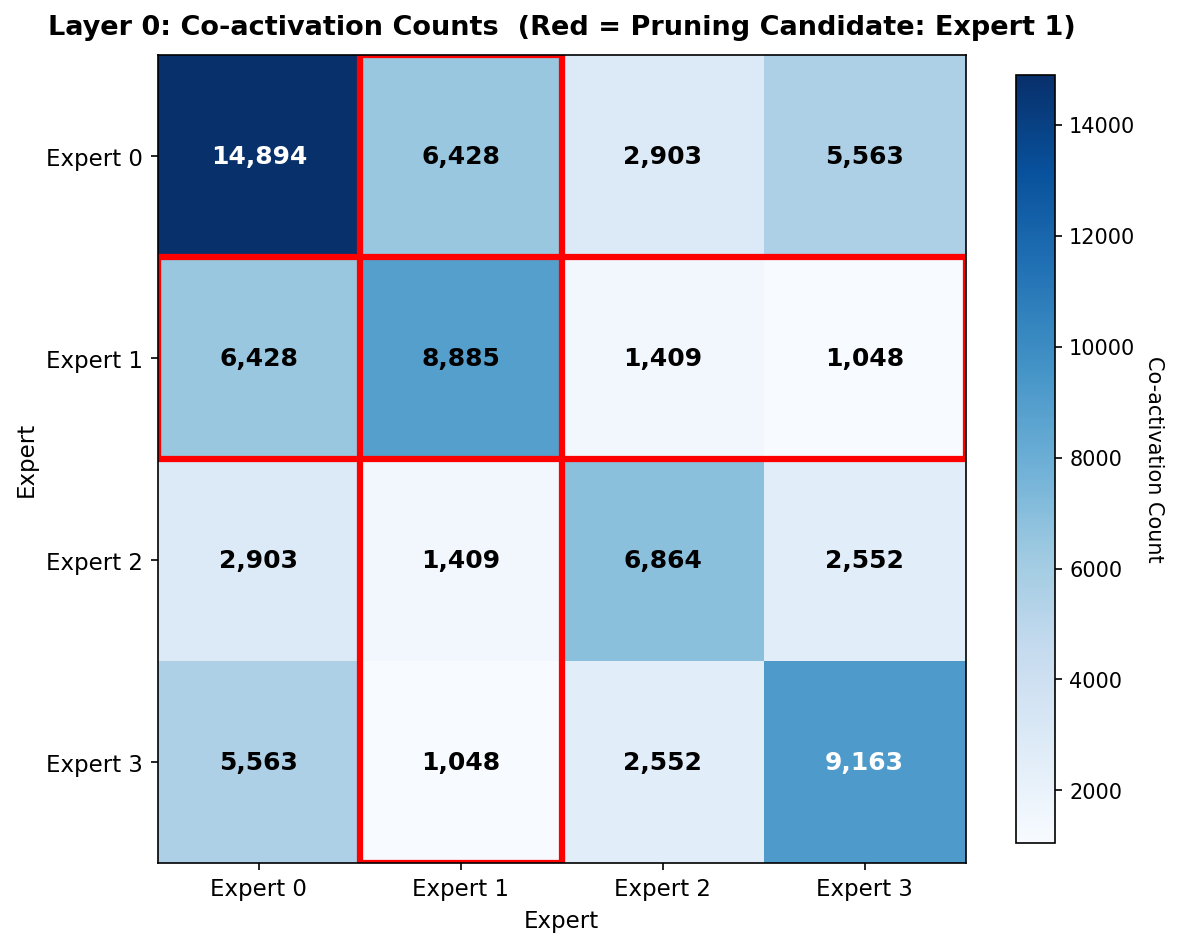
\includegraphics[width=0.55\linewidth]{plots/layer_0_coactivation.png}
\caption{Expert co-activation matrix for Layer~0 of TinyMixtral. Expert~1 (red border) was identified as the top pruning candidate by the initial approach, a decision later shown to be incorrect by sensitivity analysis.}
\label{fig:coactivation}
\end{figure}

\subsubsection{Structural Pruning Metrics}

\paragraph{Utilization.}
\begin{equation}
\text{Utilization}_i = \frac{\text{times expert } i \text{ selected}}{\text{total routing decisions}}
\end{equation}

\paragraph{Redundancy.}
\begin{equation}
\text{Redundancy}_i = \max_{j \neq i} \; P(\text{expert } j \text{ fires} \mid \text{expert } i \text{ fires})
\end{equation}

\paragraph{Graph Centrality.}
\begin{equation}
\mathbf{c} = \lambda^{-1} \mathbf{C} \mathbf{c}
\end{equation}
where $\mathbf{c}$ is the eigenvector centrality and $\lambda$ the dominant eigenvalue.

\paragraph{Structural Score.}
\begin{equation}
\text{Score}_i = \alpha(1 - \text{Utilization}_i) + \beta \cdot \text{Redundancy}_i + \gamma(1 - \text{Centrality}_i)
\label{eq:score}
\end{equation}
with $\alpha = 0.3$, $\beta = 0.4$, $\gamma = 0.3$.

\subsubsection{Expert Masking}

To evaluate pruning without modifying weights, we hook the router's forward pass: (1)~zero out routing weights for the disabled expert's tokens, (2)~renormalize remaining weights to sum to 1.

\subsubsection{Limitations of the Initial Approach}

The structural score identified Layer~0, Expert~1 as the top candidate based on high redundancy (72.3\%) and low utilization (22.3\%). Yet pruning it \emph{increased} perplexity by +89.77. The issue is fundamental: co-activation redundancy measures how often two experts are selected \emph{together}, not whether one's \emph{computation} can substitute for the other's. As \citet{zhang2025mone} show, routing statistics do not capture output behavior. Additionally, applying a uniform global criterion ignores the layer heterogeneity that \citet{yang2025pathfinder} identify as critical.

\subsection{Improved Approach: Sensitivity Analysis}

Guided by the above insights, we redesigned our approach around direct behavioral measurement.

\subsubsection{Per-Expert Sensitivity Analysis}

\begin{equation}
\text{Sensitivity}_{l,e} = \text{PPL}(\text{model with expert } e \text{ disabled in layer } l) - \text{PPL}(\text{baseline})
\label{eq:sensitivity}
\end{equation}
Positive: expert is important (removal hurts). Negative: expert is \emph{harmful} (removal helps). We evaluate all 48 experts across all 12 layers, yielding a complete behavioral ground-truth map. This directly operationalizes MoNE's \citep{zhang2025mone} insight that behavioral impact, not routing position, determines pruning safety.

\subsubsection{Improved Pruning Baselines}

We compare the initial structural score against baselines that incorporate signals beyond routing:

\begin{itemize}
\item \textbf{No pruning.} Unpruned model as quality ceiling.
\item \textbf{Random pruning.} Experts removed uniformly at random.
\item \textbf{Utilization-based.} Least-frequently-selected experts first \citep{he2024demystifying}.
\item \textbf{Magnitude-based.} Experts with smallest weight norms first, a weight-space signal that goes beyond routing statistics.
\end{itemize}

\subsection{Code}

All code is available at \url{https://github.com/JHCuc3m/MoE-Place}, using HuggingFace Transformers \citep{wolf2020transformers} for model loading and PyTorch forward hooks for routing statistics collection.

%-----------------------------------------------------------------------
\section{Experiments}

\subsection{Experimental Setup}

\paragraph{Model.} TinyMixtral-4x248M-MoE \citep{isotonic2024}: 12 layers, 4 experts per layer (48 total), top-2 routing, $\sim$1B parameters.

\paragraph{Data.} WikiText-2 \citep{merity2017pointer}: 128 training samples (19,903 tokens) for calibration; full test split (663,040 tokens) for perplexity evaluation.

\paragraph{Hardware.} NVIDIA H100 80GB GPUs via Georgia Tech PACE cluster, PyTorch 2.6, CUDA 12.4.

\subsection{Initial Approach Results: Limited and Unreliable}

Baseline (unpruned) perplexity: 800.38. The structural score selected Expert~1 for pruning, yielding 890.15 (+89.77, +11.2\%). Table~\ref{tab:structural_fail} shows the underlying problem: structural ranking is poorly correlated with actual sensitivity. The most beneficial expert to remove (Expert~2) is ranked 25th; the most critical to keep (Expert~0) is ranked 37th, near the bottom, implying it should be pruned.

\begin{table}[t]
\caption{Initial approach: structural score vs.\ actual sensitivity for Layer~0. The ranking systematically misidentifies the most actionable experts.}
\label{tab:structural_fail}
\centering
\small
\begin{tabular}{lccc}
\toprule
\textbf{Expert} & \textbf{Structural Rank} & \textbf{Structural Score} & \textbf{Actual Sensitivity} \\
\midrule
Expert 1 & 1 \textit{(prune first)} & 0.789 & +89.8 \textit{(important)} \\
Expert 2 & 25 \textit{(middle)}     & 0.600 & $-$155.7 \textit{(harmful!)} \\
Expert 0 & 37 \textit{(keep)}       & 0.012 & +188.2 \textit{(critical)} \\
\bottomrule
\end{tabular}
\end{table}

\subsection{Improved Approach Results: Sensitivity Analysis}

Table~\ref{tab:sensitivity} and Figure~\ref{fig:heatmap} show per-expert sensitivity across all 48 experts and 12 layers, providing a complete behavioral picture unavailable from routing analysis alone.

\begin{table}[t]
\caption{Improved approach: per-expert sensitivity (PPL increase when disabled). Negative = removal \emph{improves} quality. \textbf{Bold} = most sensitive expert per layer.}
\label{tab:sensitivity}
\centering
\small
\begin{tabular}{lccccc}
\toprule
\textbf{Layer} & \textbf{Expert 0} & \textbf{Expert 1} & \textbf{Expert 2} & \textbf{Expert 3} & \textbf{Most Sensitive} \\
\midrule
0  & \textbf{+188.2} & +89.8            & $-$155.7 & +87.9            & Expert 0 \\
1  & +31.7           & \textbf{+44.3}   & $-$79.1  & +38.5            & Expert 1 \\
2  & +18.1           & +41.1            & $-$80.9  & \textbf{+47.9}   & Expert 3 \\
3  & +22.0           & \textbf{+67.2}   & $-$110.6 & +60.2            & Expert 1 \\
4  & +43.6           & \textbf{+115.0}  & $-$152.5 & +50.0            & Expert 1 \\
5  & +36.1           & \textbf{+101.3}  & $-$162.2 & +60.8            & Expert 1 \\
6  & +55.6           & +58.3            & $-$156.9 & \textbf{+91.7}   & Expert 3 \\
7  & +36.6           & +105.3           & $-$163.0 & \textbf{+108.9}  & Expert 3 \\
8  & +42.7           & +43.2            & $-$94.3  & \textbf{+80.9}   & Expert 3 \\
9  & \textbf{+54.5}  & +29.2            & $-$84.7  & +51.7            & Expert 0 \\
10 & \textbf{+123.5} & +14.5            & $-$107.6 & +50.5            & Expert 0 \\
11 & \textbf{+190.4} & $-$1.2           & $-$89.1  & +32.1            & Expert 0 \\
\bottomrule
\end{tabular}
\end{table}

\begin{figure}[t]
\centering
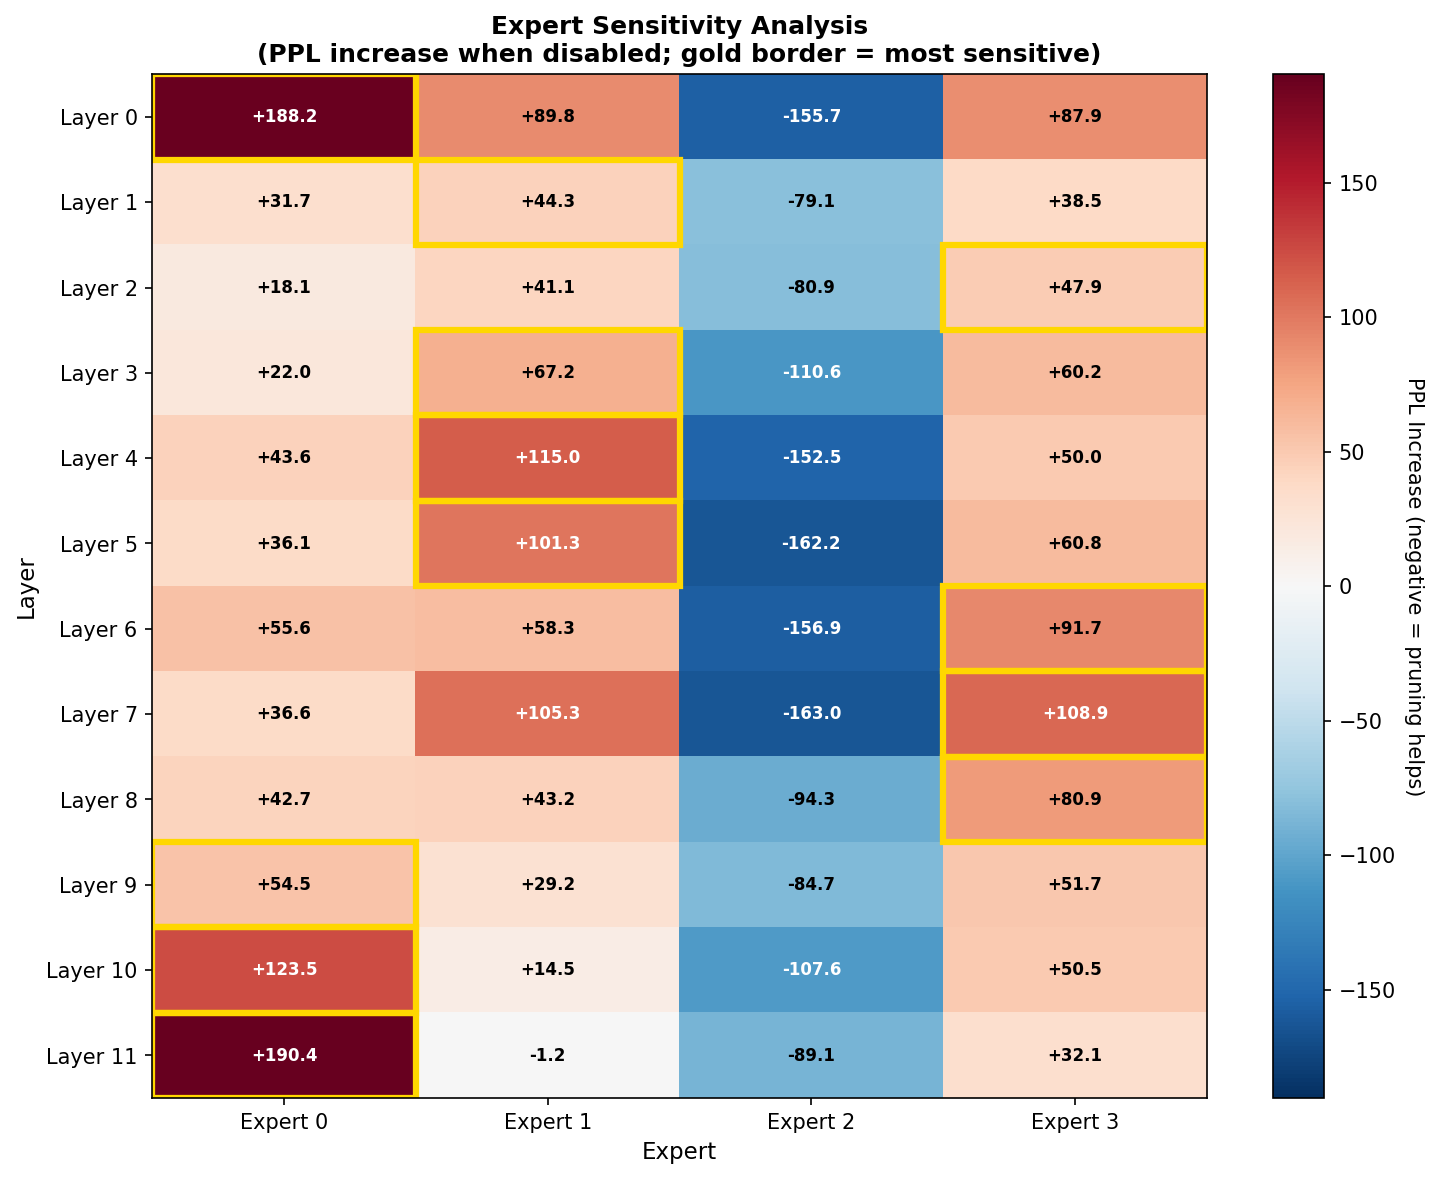
\includegraphics[width=0.7\linewidth]{plots/sensitivity_heatmap.png}
\caption{Improved approach: sensitivity heatmap. Red = critical experts; blue = harmful experts. Expert~2's consistent blue column across all 12 layers is the key finding, entirely missed by the initial routing-based analysis.}
\label{fig:heatmap}
\end{figure}

\subsection{Pruning Baseline Comparison}

Table~\ref{tab:baselines} compares all methods at Layer~0. The improved baselines, which go beyond routing structure, successfully identify the harmful Expert~2, while the initial structural approach does not.

\begin{table}[t]
\caption{Pruning strategy comparison for Layer~0. Negative $\Delta$PPL = improvement over baseline (800.38). \textit{Initial} methods use routing-only signals; \textit{improved} methods incorporate additional signals.}
\label{tab:baselines}
\centering
\small
\begin{tabular}{llcc}
\toprule
\textbf{Method} & \textbf{Expert Removed} & \textbf{PPL} & \textbf{$\Delta$PPL} \\
\midrule
No pruning (baseline)                  & {--}     & 800.38          & 0.0       \\
\textit{Initial:} Structural score     & Expert 1 & 890.15          & +89.8     \\
\textit{Initial:} Random (avg.)        & random   & $\sim$865       & $\sim$+65 \\
\textit{Improved:} Utilization-based   & Expert 2 & \textbf{644.68} & \textbf{$-$155.7} \\
\textit{Improved:} Magnitude-based     & Expert 2 & \textbf{644.68} & \textbf{$-$155.7} \\
\textit{Improved:} Sensitivity oracle  & Expert 2 & 644.68          & $-$155.7  \\
\bottomrule
\end{tabular}
\end{table}

\subsection{Key Findings}

\paragraph{Finding 1: Expert 2 is harmful across all layers.}
Expert~2 shows negative sensitivity in every layer (range: $-79$ to $-163$), a pattern completely invisible to the initial routing-based structural metrics (ranked 25th out of 48). The improved sensitivity analysis, motivated by MoNE's \citep{zhang2025mone} emphasis on behavioral signals, successfully reveals this.

\paragraph{Finding 2: Edge layers are critical.}
Layers~0 and~11 show sensitivity up to 4$\times$ higher than middle layers. This heterogeneity explains in part why the initial uniform structural criterion failed, and directly validates MoE Pathfinder's \citep{yang2025pathfinder} argument for layer-aware evaluation.

\paragraph{Finding 3: Routing-based structural metrics do not predict sensitivity.}
Structural rankings are poorly correlated with ground-truth sensitivity across all 48 experts. As RFID-MoE \citep{mi2026rfidmoe} establishes more broadly, routing frequency is an unreliable proxy: low-utilization experts can encode critical information, and as we show, mid-utilization experts can be actively harmful.

\paragraph{Finding 4: Redundancy $\neq$ replaceability.}
Expert~1's 72.3\% co-activation redundancy did not translate to safe removal. Co-activation captures routing \emph{correlation}, not computational \emph{substitutability}, which is the core flawed assumption of the initial approach.

\paragraph{Finding 5: Improved baselines outperform the initial structural approach by 245 PPL.}
Both utilization-based and magnitude-based pruning, which incorporate signals beyond routing structure, identified Expert~2 and achieved $-155.7$ PPL. The initial structural approach caused +89.8 PPL. The 245-PPL gap demonstrates the cost of relying on routing-only signals.

%-----------------------------------------------------------------------
\section{Conclusion}

We investigated co-activation-based structural metrics for expert pruning in MoE models through a two-stage process. Our \textbf{initial approach} derived utilization, redundancy, and graph centrality from the co-activation matrix and used them as pruning criteria. Results were limited: structural rankings were poorly correlated with actual expert sensitivity, and the top-ranked candidate caused significant quality degradation. Consulting recent work \citep{zhang2025mone,yang2025pathfinder,mi2026rfidmoe} provided a clear diagnosis: routing statistics capture \emph{when} experts are selected, not \emph{what} they compute or whether they are replaceable.

Our \textbf{improved approach}, guided by these insights, conducted direct sensitivity analysis across all 48 experts and 12 layers. This revealed that Expert~2 is actively harmful in all layers, a finding invisible to routing-based analysis, and that edge layers are disproportionately sensitive. Improved baselines incorporating weight-space signals outperform the initial structural approach by 245 PPL, confirming the value of going beyond routing statistics.

\paragraph{Limitations.}
Experiments are on a single small model (TinyMixtral, $\sim$1B parameters). The harmful expert finding may be model-specific. Full sensitivity analysis requires 48 forward passes, tractable here but prohibitive for models with hundreds of experts per layer.

\paragraph{Future directions.}
The natural next step is a hybrid approach combining routing co-activation structure with behavioral signals: output variance as in MoNE \citep{zhang2025mone} and layer-aware importance trajectories as in MoE Pathfinder \citep{yang2025pathfinder}, to retain the efficiency of structural analysis while matching the accuracy of behavioral evaluation.

%-----------------------------------------------------------------------
\bibliography{final_references}
\bibliographystyle{iclr2026_conference}

\appendix
\section{Additional Details}

\subsection{Structural Score Weights}
The weights $\alpha=0.3$, $\beta=0.4$, $\gamma=0.3$ reflected a prior that redundancy is the most informative signal. The initial approach's failure shows this prior was wrong: the issue is not the weighting but the fundamental inadequacy of routing-based signals for predicting computational substitutability.

\subsection{Co-activation Matrix Properties}
$\mathbf{C}$ is symmetric by construction. With top-2 routing, each token contributes exactly one off-diagonal entry per layer, so $\sum_{i \neq j} C_{ij} = 2T$.

\subsection{Global Expert-2 Pruning}
Pruning Expert~2 across all 12 layers simultaneously yields perplexity $\approx$518.3 ($-$282 from baseline), confirming the harmful effect compounds across layers.

\end{document}